\section{Information and Entropy Maximization}
\label{sec:Information and Entropy Maximization}
\begin{rem}
  Entropy and mutual information are useful quantities for characterizing
the nature and efficiency of neural encoding and selectivity. Often, in addition to such characterizations, we seek to understand the
computational implications of an observed response selectivity. For example, we might
ask whether neural responses to natural stimuli are optimized to convey as
much information as possible. This hypothesis can be tested by computing
the response characteristics that maximize the mutual information con-
veyed about naturally occurring stimuli and comparing the results with
responses observed experimentally.
\end{rem}

%\begin{exm}
  
%\end{exm}

\begin{rem}
  Because the mutual information is the full response entropy minus the
noise entropy, maximizing the information involves a compromise. We
must make the response entropy as large as possible without allowing the
noise entropy to get too big. If the noise entropy is small, maximizing
the response entropy, subject to an appropriate constraint, maximizes the
mutual information to a good approximation. We therefore begin our discussion by studying how response entropy can be maximized. Later in the
discussion, we will consider the effects of noise entropy.
\end{rem}
\begin{rem}
  Constraints play a crucial role in this analysis. We have already seen that
the theoretical information-carrying capacity associated with a continuous
firing rate is limited only by the resolution with which the firing rate can be
defined.????????????????????????????????
\end{rem}
\subsection{Entropy Maximization for a Single Neuron}
\begin{asm}
 During the maximization process, the resolution $r$ is held fixed, so the
 $\log_2\Delta r$ term remains constant, and it can be ignored. As a
 result, it will not generally appear in the following equations.
\end{asm}

\begin{rem}
  To maximize the response entropy, we must find a probability density $p[r]$
that makes the integral in equation \ref{equ:4.17} as large as possible while satisfying whatever constraints we impose. One constraint that always
applies in entropy maximization is that the integral of the
probability density must be 1.
\end{rem}


\begin{prop}
  \label{prop:solveForMaximum}
  Suppose that the neuron in question has a maximum firing rate of $r_{\max}$. Then, 
  \begin{equation}
    \label{equ:4.22}
    p[r]=\frac{1}{r_{{\max}}}
  \end{equation}
  solves
  \begin{equation}
    \label{equ:4.20}
    \max\limits_{p[r]} \int_{0}^{r_{{\max}}}p[r]\log_2p[r],\ s.t.\ \int_{0}^{r_{{\max}}}p[r]dr=1.
  \end{equation}
  The entropy for this probability density, for finite firing rate resolution $\Delta r$, is
  \begin{equation}
    \label{equ:4.23}
    H=\log_2\left( \frac{r_{{\max}}}{\Delta r} \right).
  \end{equation}
  \begin{proof}
    Equation \ref{equ:4.22} is from Lagrange multipliers and the same way to compute the functional derivative as Proposition \ref{prop:OptimalLinearKernel}. Thus, $H=\log_2r_{{\max}}-\log_2\Delta r=\log_2\left( \frac{r_{{\max}}}{\Delta r} \right)$.
  \end{proof}
\end{prop}

\begin{rem}
  Equation \ref{equ:4.22} is independent of $r$ and is the basis of a signal-processing technique called \emph{histogram equalization}. Applied to neural responses, this is a procedure for tailoring the neuronal selectivity so that $p[r]=1/r_{{\max}}$ in response to a set of stimuli over which the entropy is to be maximized.
\end{rem}
\begin{prop}
  \label{prop:tuningCurveForMaximum}
  Suppose a neuron responds to a stimulus characterized by the parameter s by firing at a rate $r=f(s)$. If the response probability density takes its optimal value, $p[r] = 1/r_{\max}$, the corresponding turning curve in the case of a monotonically increasing response is
  \begin{equation}
    \label{equ:4.25}
    f(s)=r_{{\max}}\int_{s_{\min}}^sp[s']ds',
  \end{equation}
  where $s_{\min}$ is the minimum value of s, which is assumed to generate no response.
  \begin{proof}
    For small $\Delta s$, the probability that the continuous stimulus variable falls in the range between $s$ and $s+\Delta s$ is given in terms of the stimulus probability density by $p[s]\Delta s$. This produces a response that falls in the range between $f(s+\Delta s)$ and $f(s)$. When $p[r]=1/r_{{\max}}$, the probability that the response falls within this range is $|f(s+\Delta s)-f(s)|/r_{{\max}}$. Setting these two probabilities equal to each other, we find that
    \begin{equation}
      \label{equ:equal probability}
      \frac{|f(s+\Delta s)-f(s)|}{r_{{\max}}}=p[s]\Delta s.
    \end{equation}
    Because of the monotonically increasing response so that $f(s+\Delta s)>f(s)$ for positive $\Delta s$. Then,in the limit $\Delta s\rightarrow 0$, the equalization condition becomes
    \begin{equation}
      \frac{df}{ds}=r_{{\max}}p[s],
    \end{equation}
    which has the solution Equation \ref{equ:4.25}.
  \end{proof}
\end{prop}
\begin{rem}
  In the case of Proposition \ref{prop:tuningCurveForMaximum}, entropy maximization requires that the average firing rate of the responding neuron be proportional to the integral of the probability density of the stimulus.
\end{rem}

\begin{exm}
  \label{exm:flyEntropyMaximize}
  The large monopolar cell (LMC) in the visual system of the fly responds to contrast, and the following figure shows that contrast response of the fly LMC (data points) compared to the integral of the natural contrast probability distribution (solid curve). The relative response is the amplitude of the membrane potential fluctuation produced by the onset of a light or dark image with a given level of contrast divided by the maximum response. Contrast is defined relative to the background level of illumination.
\begin{center}
    \label{fig:4-2}
  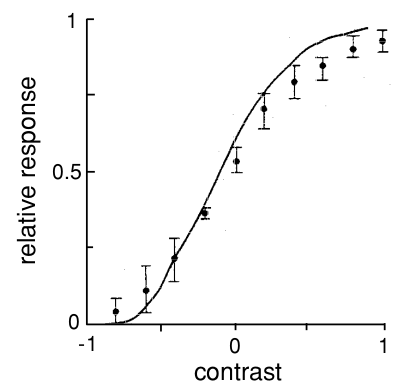
\includegraphics[scale = 0.35]{./png/4-2}
\end{center}
The response as a function of contrast is very close to the integrated probability density, suggesting that the LMC is using a maximum entropy encoding.
\end{exm}

\begin{rem}
  These responses in Example \ref{exm:flyEntropyMaximize} are measured as membrane potential fluctuation amplitudes, not as firing rates, but the analysis presented can be applied without modification.
\end{rem}


\begin{rem}
  Even though neurons have maximum firing rates, the constraint $r\leq r_{{\max}}$
  may not always be the factor that limits the entropy. For example,
  the average firing rate of the neuron may be constrained to values
  much less than $r_{{\max}}$, or the variance of the firing rate might be constrained.
\end{rem}
\begin{exc}
  Show that the entropy-maximizing probability density is an exponential, if the average firing rate is constrained to a fixed value.
\end{exc}

\begin{exc}
  Show that the probability density that maximizes the entropy subject to constraints on the firing rate and its variance is a Gaussian.
\end{exc}


\subsection{Populations of Neurons}
\begin{rem}
  When a population of neurons encodes a stimulus, optimizing their individual response properties will not necessarily lead to an optimized population response. Optimizing individual responses could result in a highly redundant population representation in which different neurons encode the same information.
\end{rem}

\begin{fac}
  Entropy maximization for a population requires that the neurons convey independent pieces of information (i.e., they must have different response selectivities).
\end{fac}

\begin{ntn}
  Let the vector $\mathbf{r}$ with components $r_a$ for $a=1,2,\cdots,N$ denote the firing rates for a population of $N$ neurons, measured with resolution $\Delta r$. 
\end{ntn}

\begin{thm}
  If $p[\mathbf{r}]$ is the probability of evoking a population response characterized by the vector $\mathbf{r}$, the entropy for the entire
population response is
\begin{equation}
  \label{equ:4.26}
  H=-\int{p[\mathbf{r}]\log_2p[r]d\mathbf{r}}-N\log_2\Delta r.
\end{equation}
\end{thm}

\begin{prop}
  Along with the full population entropy of Equation \ref{equ:4.26}, we
  can also consider the entropy associated with individual neurons
  within the population. If $p[r_a]=\int\prod_{b\neq
    a}p[\mathbf{r}]dr_b$ is the probability density for response $r_{a}$ from
  neuron $a$, its entropy is
  \begin{equation}
    \begin{aligned}
       \label{equ:4.27}
    H_a&=-\int{p[r_a]\log_2p[r_a]dr_a}-\log_2{\Delta r}\\
        &=-\int{p[\mathbf{r}]\log_2p[r_a]d\mathbf{r}}-\log_2{\Delta r}.
    \end{aligned}
  \end{equation}
\end{prop}

\begin{prop}
  \label{prop:indpendent population entropy}
  The true population entropy can never be greater than the sum of these
  individual neuron entropies over the entire population,
  \begin{equation}
    \label{equ:4.28}
    H\leq \sum\limits_{a}{H_a}.
  \end{equation}
  \begin{proof}
    To prove this, we note that the difference between the full entropy and the
    sum of individual neuron entropies is
    \begin{equation*}
      \label{equ:4.29}
      \sum\limits_{a}H_a-H=\int{p[\mathbf{r}]\log_2\left(\frac{p[\mathbf{r}]}{\prod_ap_a[r_a]}\right)\geq0}.
    \end{equation*}
    The inequality follows from the fact that the middle expression is the KL
divergence between the probability distributions $p[r]$ and a $p[r_a]$, and a
KL divergence is always nonnegative. Equality holds only if
\begin{equation}
  \label{equ:4.30}
  p[\mathbf{r}]=\prod_ap[r_a],
\end{equation}
that is, if the responses of the neurons are statistically independent. Thus,
the full response entropy is never greater than the sum of the entropies of
the individual neurons in the population, and it reaches the limiting value
when Equation \ref{equ:4.30} is satisfied.
  \end{proof}
\end{prop}

\begin{defn}
  \label{defn:factorial code}
  A code that satisfies this condition is called
a \emph{factorial code} because the probability factorizes into a product of single
neuron probabilities.
\end{defn}

\begin{rem}
  When the population-response probability density
factorizes, this implies that the individual neurons respond independently.
The entropy difference in Equation \ref{equ:4.29} has been suggested as a measure
of redundancy.
\end{rem}
\begin{prop}
  Combining the result in proposition \ref{prop:indpendent population entropy} with the results of the previous section, we con-
clude that the maximum population-response entropy can be achieved by
satisfying two conditions:
\begin{enumerate}
\item The individual neurons must respond in-
dependently, which means that $ p[\mathbf{r}]=\prod_ap[r_a]$ must
factorize.
\item If the same
constraint is imposed on every neuron, the second condition implies that
every neuron must have the same response probability density. In other
words, $p[r_a]$ must be the same for all a values, a property called probability
equalization.
\end{enumerate}
\end{prop}

\begin{rem}
  We proceed
by considering factorization and probability equalization as general principles of entropy maximization, without imposing explicit constraints.
\end{rem}

\begin{rem}
  Exact factorization and probability equalization are difficult to achieve,
especially if the form of the neural response is restricted. These goals are
likely to be impossible to achieve, for example, if the neural responses are
modeled as having a linear relation to the stimulus?????????. 
\end{rem}

\begin{thm}
  A more modest goal is to require that the lowest-order moments of the population-response probability distribution match those of a fully factorized and equalized
distribution. If the individual response probability distributions are
equal, the average firing rates and firing rate variances will be the
same for all neurons.
\begin{equation}
  \label{equ:variance}
  \left\langle r_a \right\rangle=\left\langle r \right\rangle
 \quad \text{and}\quad
  \left\langle (r_a-\left\langle r \right\rangle)^2 \right\rangle=\sigma_r^{2}.
\end{equation}
for all $a$.
Furthermore, the covariance
matrix for a factorized and probability-equalized population distribution
is proportional to the identity matrix,
\begin{equation}
  \label{equ:4.31}
  Q_{ab}=\int{p[\mathbf{r}]\left( r_a-\left\langle r \right\rangle \right)\left( r_b-\left\langle r \right\rangle \right)d\mathbf{r}}=\sigma_r^2\delta_{ab}.
\end{equation}
\end{thm}

\begin{rem}
  Finding response distributions that satisfy only the decorrelation and vari-
ance equalization condition of equation 4.31 is usually tractable. In the fol-
lowing examples, we restrict ourselves to this easier task. This maximizes
the entropy only if the statistics of the responses are Gaussian, but it is
a reasonable procedure even in a non-Gaussian case, because it typically
reduces the redundancy in the population code and spreads the load of
information transmission equally among the neurons.
\end{rem}

\subsection{Application to Retinal Ganglion Cell Receptive Fields}
\begin{asm}
  Entropy and information maximization have been used to explain proper-
ties of visual receptive fields in the retina, LGN, and primary visual cor-
tex. The basic assumption is that these receptive fields serve to maximize
the amount of information that the associated neural responses convey
about natural visual scenes in the presence of noise.
\end{asm}
\begin{rem}
  Information theoret-
ical analyses are sensitive to the statistical properties of the stimuli being
represented, so the statistics of natural scenes play an important role in
these studies. Natural scenes exhibit substantial spatial and temporal re-
dundancy. Maximizing the information conveyed requires removing this
redundancy from the neural responses.
\end{rem}
\begin{rem}
  It should be kept in mind that the information maximization approach
sets limited goals and requires strong assumptions about the nature of the
constraints relevant to the nervous system. In addition, the approach ana-
lyzes only the representational properties of neural responses and ignores
the computational goals of the visual system, such as object recognition
or target tracking. Never-
theless, the principle of information maximization is quite successful at
accounting for properties of receptive fields early in the visual pathway.
\end{rem}

\begin{ntn}
   In chapter 2, a visual image was defined by a contrast function $s(x,y,t)$
with a trial-averaged value of 0. For the calculations we present here, it
is more convenient to express the $x$ and $y$ coordinates for locations on the viewing screen in terms of a single vector $\vec{x}=(x,y)$, or sometimes $\vec{y}=(x,y)$.
\end{ntn}
\begin{thm}
The linear estimate of the response of a visual neuron discussed in chapter 2 can be written as
\begin{equation}
  \label{equ:4.32}
  L(t)=\int_0^{\infty}\int{D(\vec{x},\tau)s(\vec{x},t-\tau)d\vec{x}d\tau}.
\end{equation}
\end{thm}
\begin{prop}
  If the space-time receptive field $D(\vec{x},\tau)$ is separable, $D(\vec{x},\tau)=D_{s}(\vec{x})D_t(\tau)$,
and we can rewrite $L(t)$ as the product of integrals involving temporal
and spatial filters. To keep the notation simple, we assume that the stimu-
lus can also be separated, so that
$s(\vec{x},\tau)=s_s(\vec{x})s_t(t)$. Then,
\begin{equation}
  \label{equ:separable space-time receptive field }
 L(t)=L_sL_t(t), 
\end{equation}
where
\begin{equation}
  \label{equ:4.33}
  L_s=\int{D_s(\vec{x})s_s(\vec{x})d\vec{x}}
\end{equation}
and
\begin{equation}
  \label{equ:4.34}
  L_t(t)=\int_0^{\infty}D_t(\tau)s_t(t-\tau)d\tau.
\end{equation}
\end{prop}

\begin{rem}
  In the following, we analyze the spatial and temporal components, $D_s$ and
$D_t$, separately by considering the information-carrying capacity of $L_s$ and
$L_t$.
\end{rem}

\begin{asm}
  \label{asm:homogeneity}
  To derive appropriately optimal spatial filters, we consider an array of
retinal ganglion cells with receptive fields covering a small patch of the
retina.We assume that the statistics of the input which is most
effective are spatially (and temporally) stationary or
translation-invariant. This means that all locations
and directions in space (and all times), at least within the patch we con-
sider, are equivalent. This equivalence allows us to give all of the receptive
fields the same spatial structure, with the receptive fields of different cells
merely being shifted to different points within the visual field.
\end{asm}

\begin{ntn}
  Note that we are labeling the neurons by the locations $\vec{a}$ of the centers of
their receptive fields rather than by an integer index such as $i$. This is a
convenient labeling scheme that allows sums over neurons to be replaced
by sums over parameters describing their receptive fields.The vectors
$\vec{a}$ for the different neurons take on discrete values corresponding to the
different neurons in the population.
\end{ntn}
\begin{prop}
  Based on the above assumptions, we write the spatial kernel describing a retinal ganglion cell with receptive
field centered at the point $\vec{a}$ as $D_s(\vec{x}-\vec{a})$. The linear response of this cell is
then
\begin{equation}
  \label{equ:4.35}
  L_s(\vec{a})=\int{D_s(\vec{x})-\vec{a}s_s(\vec{x})d\vec{x}}.
\end{equation}
\end{prop}

\begin{rem}
  If many neurons are being considered,
these discrete vectors may fill the range of receptive field locations quite
densely. In this case, it is reasonable to approximate the large but
discrete set of $\vec{a}$ values with a vector $\vec{a}$ that is
allowed to vary continuously. In
other words, as an approximation, we proceed as if there were a neuron
corresponding to every continuous value of $\vec{a}$. This allows us
to treat as a function of $\vec{a}$ and to replace sums over neurons
with integrals over $\vec{a}$. In the case we are considering, the receptive fields of retinal ganglion
cells cover the retina densely, with many receptive fields overlapping each
point on the retina, so the replacement of discrete sums over neurons with
continuous integrals over $\vec{a}$ is quite accurate.
\end{rem}

\subsection{The Whitening Filter}
The relevant correlation is the average, over all stimuli, of the product of the linear responses
of two cells, with receptive fields centered at $\vec{a}$ and
$\vec{b}$,
\begin{equation}
  \begin{aligned}
     \label{equ:4.366}
  Q_{\text{LL}}(\vec{a},\vec{b})&=\left\langle L_s(\vec{a})L_s(\vec{b})
  \right\rangle\\
  &=\int{D_s(\vec{x})-\vec{a})D_s(\vec{y})-\vec{b})\left\langle s_s(\vec{x})s_s(\vec{y}) \right\rangle d\vec{x}d\vec{y}}.
  \end{aligned}
\end{equation}
Here the average, denoted by angle brackets, is not over trials but over the
set of natural scenes for which we believe the receptive field is
optimized.
\begin{prop}
  By analogy with Equation \ref{equ:4.31}, decorrelation and variance equalization of
the different retinal ganglion cells, when $\vec{a}$ and $\vec{a}$ are taken to be continuous
variables, require that we set this correlation function proportional to a $\delta$
function,
\begin{equation}
  \label{equ:4.37}
  Q_{\text{LL}}(\vec{a},\vec{b})=\sigma_L^2\delta(\vec{a}-\vec{b}).
\end{equation}
which is the continuous variable analog of making a discrete correlation ma-
trix proportional to the identity matrix (Equation \ref{equ:4.31}).
\end{prop}

\begin{thm}
  Our assumption of homogeneity \ref{asm:homogeneity}
  implies that $\left\langle s_s(\vec{x})s_s(\vec{y})\right\rangle$ is only a function of the vector difference $\vec{x}-\vec{y}$ (actually, if all directions are equivalent, it is only a function of the magnitude $\vec{x}-\vec{y}$), and we write it as
  \begin{equation}
    \label{equ:4.38}
    Q_{ss}(\vec{x}-\vec{y})=\left\langle s_s(\vec{x})s_s(\vec{y})\right\rangle.
  \end{equation}
\end{thm}


\begin{thm}
  The optimal receptive field filter (entropy maximization) for receptive field filter is
  \begin{equation}
    \label{equ:4.42}
    \left| \tilde{D}_s(\vec{\kappa}) \right|=\frac{\sigma_L}{\sqrt{\tilde{Q}_{ss}(\vec{\kappa})}}.
  \end{equation}
  \begin{proof}
    To determine the form of the receptive field filter that is optimal, we must
    solve equation \ref{equ:4.37} for $D_s$. This is done by expressing $D_s$ and $Q_{ss}$ in terms of their Fourier transforms $\tilde{D}_s$ an  $\tilde{Q}_{ss}$,
    \begin{equation}
      \begin{aligned}
      \label{equ:4.394.40}
        D_s(\vec{x}-\vec{a})&=\frac{1}{4\pi^{2}}\int{\exp \left( -i\vec{\kappa} \cdot(\vec{x}-\vec{a}) \right)\tilde{D}_s(\vec{\kappa})d\vec{\kappa}}\\
         QQ_{ss}(\vec{x}-\vec{y})&=\frac{1}{4\pi^2}\int{\exp \left( -i\vec{\kappa} \cdot(\vec{x}-\vec{y}) \right)\tilde{Q}_{ss}(\vec{\kappa})d\vec{\kappa}}.   
              \end{aligned}
            \end{equation}
            where $\tilde{Q}_{ss}$ is real and nonnegative, is also called the stimulus power spectrum.
            In terms of these Fourier transforms, Equation \ref{equ:4.37} becomes
            \begin{equation}
              \label{equ:4.41}
            \left| \tilde{D}_s(\vec{\kappa}) \right|^2\tilde{Q}_{ss}(\vec{\kappa})=\sigma_L^2.
            \end{equation}
          \end{proof}
\end{thm}\qedhere
\begin{rem}
  The linear kernel described by equation 4.42 exactly compensates for
whatever dependence the Fourier transform of the stimulus correlation 
function has on the spatial frequency $\vec{\kappa}$, making the product $\tilde{Q}_{ss}(\vec{\kappa})\left| \tilde{D}_s(\vec{\kappa})  \right|^{2}$ independent of $\vec{\kappa}$. This product is the power spectrum of $L$. 
\end{rem}

\begin{defn}
  The output of the optimal filter has a power spectrum that is independent of spatial fre-
quency, and therefore has the same characteristics as white noise. There-
fore, the kernel in Equation \ref{equ:4.42} is called a whitening filter.
\end{defn}

\begin{rem}
  Different spatial frequencies act independently in a linear system,????????????????????????
\end{rem}

\begin{rem}
  The calculation we have performed determines only the amplitude $\left| \tilde{D}_s(\vec{\kappa}) \right|$
and not $\tilde{D}_s(\vec{\kappa})$ itself. Thus, decorrelation and variance equalization do
not uniquely specify the form of the linear kernel. We study some consequences of the freedom to choose different linear kernels satisfying Equation \ref{equ:4.42} later in the chapter.
\end{rem}

\begin{exm}
  The spatial correlation function for natural scenes has been measured,
 with the result that $\tilde{Q}_{ss}(\vec{\kappa})$ is proportional to $1/\left| \vec{\kappa} \right|^2$ over the range it has
 been evaluated. The behavior near $\vec{\kappa}=0$ is not well established, but the divergence of $1/\left| \vec{\kappa} \right|^2$  near $\vec{\kappa}=0$ can be removed by setting $\tilde{Q}_{ss}(\vec{\kappa})$ proportional to $1/(\left| \vec{\kappa} \right|^2+\kappa_0^{2})$  where $\kappa_0$ is a constant.
 The stimuli of interest in the calculation of retinal ganglion receptive fields are natural images as they appear on the retina, not in the photographs from which the natural scenes statistics are measured. An additional factor must be included in $\tilde{Q}_{ss}(\vec{\kappa})$ to account for filtering introduced by the optics of the eye (the optical modulation transfer function). A simple model of the optical modulation transfer function results in an exponential correction to the stimulus correlation function,
 \begin{equation}
   \label{equ:4.43}
   \tilde{Q}_{ss}(\vec{\kappa})\propto \frac{\exp(-\alpha\left| \vec{\kappa} \right|)}{\left| \vec{\kappa} \right|^2+\kappa_0^{2}},
 \end{equation}
with $\alpha$ a parameter. Substituting this into Equation \ref{equ:4.42} gives the rather
eculiar result that the amplitude  $\tilde{D}_s(\vec{\kappa})$, being proportional to the inverse of the square root of $ \tilde{Q}_{ss}$, is predicted to grow exponentially for large $\left| \vec{\kappa} \right|$.
\end{exm}

\begin{thm}
  \emph{Whitening filters} maximize entropy by equalizing the distribution of
response power over the entire spatial frequency range.
\end{thm}

\begin{rem}
  High spatial frequency components of images are relatively rare in natural scenes and,
even if they occur, are greatly attenuated by the eye. The whitening filter
compensates for this by boosting the responses to high spatial frequencies. Although this is the result of the entropy maximization calculation, it is not a good strategy to use in an unrestricted way for visual processing.
\end{rem}

\begin{rem}
  Real inputs to retinal ganglion cells involve a mixture of true signal and noise
coming from biophysical sources in the retina. At high spatial frequencies,
for which the true signal is weak, inputs to retinal ganglion cells are likely
to be dominated by noise, especially in low-light conditions. Boosting the
amplitude of this noise-dominated input and transmitting it to the brain is
not an efficient visual encoding strategy. The problem of excessive boosting of responses at high spatial frequency arises in the entropy maximization calculation because no distinction has
been made between the entropy coming from true signals and that coming from noise.
\end{rem}



\subsection{Filtering Input Noise}
\begin{rem}
  To correct the problem caused by noise, we should maximize the information
transmitted by the retinal ganglion cells about natural scenes, rather than
maximize the entropy. A full information-maximization calculation of the
receptive field properties of retinal ganglion cells can be performed, but
this requires introducing a number of assumptions about the constraints
that are relevant, and it is not entirely obvious what these constraints
should be. Instead, we will follow an approximate procedure that pre-
filters the input to eliminate as much noise as possible, and then uses the
results of this section to maximize the entropy of a linear filter acting on
the prefiltered input signal
\end{rem}

\begin{asm}
  Suppose that the visual stimulus on the retina is the sum of the
  true stimulus $s_{s}\vec{x}$   that should be conveyed to the brain
  and a noise term $\eta(\vec{x})$ that reflects image distortion,
  photoreceptor noise, and other signals that are not worth conveying beyond the retina.
\end{asm}

\begin{thm}
  To deal with such a mixed input
signal, we express the Fourier transform of the linear kernel
$\tilde{D}_s(\vec{\kappa})$ as a product of two terms: a noise filter,
$\tilde{D}_{\eta}(\vec{\kappa})$, that eliminates as much of the
noise as possible; and a whitening filter,
$\tilde{D}_{w}(\vec{\kappa})$, that satisfies Equation (\ref{equ:4.42}).
The Fourier transform of the complete filter is then
\begin{equation}
  \label{equ:linear kernel}
  \tilde{D}_s(\vec{\kappa})=\tilde{D}_{w}(\vec{\kappa})\tilde{D}_{\eta}(\vec{\kappa}).
\end{equation}
\end{thm}

\begin{asm}
  we assume that the signal and noise
terms are uncorrelated, so that $\left\langle s_s(\vec{x})\eta(\vec{y}) \right\rangle=0$.
\end{asm}

\begin{thm}
  The optimal noise filter is real and
given, in terms of the Fourier transforms of $Q_{ss}$ and
$Q_{\eta\eta}$, by
\begin{equation}
  \label{equ:4.46}
  \tilde{D}_{\eta}(\vec{\kappa}) = \frac{\tilde{Q}_{ss}(\vec{\kappa})}{\tilde{Q}_{ss}(\vec{\kappa}) + \tilde{Q}_{\eta\eta}(\vec{\kappa})}.
\end{equation}
\begin{proof}
    To determine the form of the noise filter, we demand that when it is applied to the total input $s_{s}(\vec{x})+\eta(\vec{x})$, the result is
as close to the signal part of the input, $s_{s}(\vec{x})$, as
possible.
  The relevant cross-
  correlation for this problem is
\begin{equation}
  \label{equ:4.44}
  \left\langle (s_{s}(\vec{x})+\eta(\vec{x}))s_{s}(\vec{y}) \right\rangle = Q_{ss}(\vec{x}-\vec{y}),
\end{equation}
and the autocorrelation is
\begin{equation}
  \label{equ:4.45}
  \left\langle (s_{s}(\vec{x})+\eta(\vec{x}))(s_{s}(\vec{y}) + \eta(\vec{y}))\right\rangle = Q_{ss}(\vec{x}-\vec{y}) + Q_{\eta \eta}(\vec{x}-\vec{y}),
\end{equation}
where $Q_{ss}$ and $Q_{\eta\eta}$ are, respectively, the stimulus and noise autocorrelations functions.
 The problem is to minimize the average
squared difference between the filtered noisy signal and the true
signal. The general solution is that the Fourier transform of the optimal filter is the
Fourier transform of the cross-correlation between the quantity being filtered and the quantity being approximated divided by the Fourier transform of the autocorrelation of the quantity being filtered.
\end{proof}
\end{thm}

\begin{thm}
  the noise filter is designed so that its output matches the signal as
closely as possible, we make the approximation of using the same whiten-
ing filter as before (Equation \ref{equ:4.42}). Combining the two, we
find that
\begin{equation}
  \label{equ:4.47}
  \left| \tilde{D}_{s}(\vec{\kappa}) \right| \propto \frac{\sigma_{L}\sqrt{\tilde{Q}_{ss}(\vec{\kappa})}}{\tilde{Q}_{ss}(\vec{\kappa}) + \tilde{Q}_{\eta\eta}(\vec{\kappa})}.
\end{equation}
\end{thm}

\begin{exm}
  Linear kernels resulting from Equation \ref{equ:4.47}, using Equation \ref{equ:4.43} for the
stimulus correlation function, are plotted in figure A and B. For these figures,
we have assumed that the input noise is white so that
$\tilde{Q}_{\eta\eta}(\vec{\kappa})$ is independent of
$\vec{\kappa}$. The two figures descirbes are receptive field properties predicted by entropy maximization and noise
suppression of responses to natural images.\\

Both the amplitude of the Fourier transform of the
kernel (figure A) and the actual spatial kernel
$\tilde{D}_{s}(\vec{\kappa})$ (figure B) are plotted under conditions of low and high noise. The linear kernels in figure B  have been
constructed by assuming that $\tilde{D}_{s}(\vec{\kappa})$ satisfies Equation \ref{equ:4.47} and is real, which
minimizes the spatial extent of the resulting receptive field. The resulting
function $D_s(\vec{x})$ is radially symmetric, so it depends only on
the distance $\left| \vec{x} \right|$ from the center of the receptive field to the
point $\vec{x}$, and this radial dependence is plotted in figure
B. Under low noise conditions (solid lines in figure), the linear kernel has a bandpass character and the predicted
receptive field has a center-surround structure, which matches the retinal
ganglion receptive fields shown in chapter 2.\\

This structure eliminates one major source of redundancy in natural
scenes: the strong similarity of neighboring inputs owing to the
predominance of low spatial frequencies in images. When the noise
level is high (dashed lines in figure 4.3), the structure of the
optimal receptive field is different. In spatial frequency terms, the
filter is now low-pass, and the receptive field loses its surround. This structure
averages over neighboring pixels to extract the true signal obscured
by the the uncorrelated noise. In the retina, we expect the signal-to-noise ratio to be
controlled by the level of ambient light, with low levels of illumination
corresponding to the high-noise case. The predicted change in the recep-
tive fields at low illumination (high noise) matches what actually happens
in the retina. At low light levels, circuitry changes within the retina re-
move the opposing surrounds from retinal ganglion cell receptive
fields.
\begin{center}
    \label{fig:4-3}
  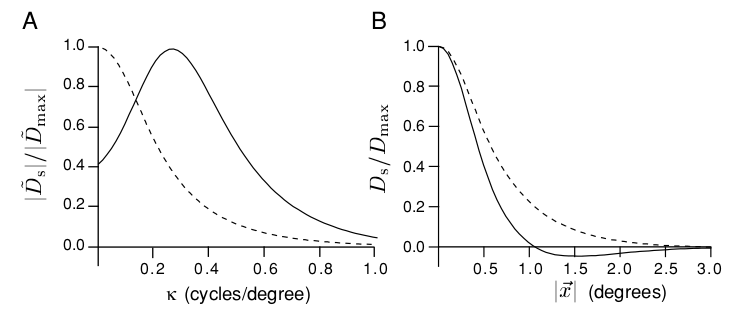
\includegraphics[scale = 0.35]{./png/4-3}
\end{center}
\end{exm}


\subsection{Temporal Processing in the LGN}
\begin{rem}
  Natural images tend to change relatively slowly over time. This means
that there is substantial redundancy in the succession of natural images,
suggesting an opportunity for efficient temporal filtering to complement
efficient spatial filtering.
\end{rem}
\begin{rem}
  An analysis similar to that of the previous section
can be performed to account for the temporal receptive fields of visually
responsive neurons early in the visual pathway.
\end{rem}

\begin{thm}
  Recall that the predicted
linear temporal response is given by $L_t(t)$, as expressed in
Equation \ref{equ:4.34}.The analog of Equation \ref{equ:4.37} for
temporal decorrelation and variance equalization is
\begin{equation}
  \label{equ:4.48}
  \left\langle L_{t}(t)L_{t}(t') \right\rangle = \sigma_{L}^{2}\delta(t-t').
\end{equation}
which is mathematically identical to equation \ref{equ:4.37} except that the role of
the spatial variables $\vec{a}$ and $\vec{b}$ has been replaced by
the temporal variables $t$ and $t'$.
\end{thm}

\begin{thm}
  The analysis proceeds exactly as above, and the optimal filter is
the product of a noise filter and a temporal whitening filter, as before. The
temporal linear kernel $D_t(\tau)$ is written in terms of its Fourier
transform,
\begin{equation}
  \label{equ:4.49}
  D_{t}(\tau) = \frac{1}{2\pi}\int \exp(-i\omega\tau)\tilde{D}_{t}(\omega)d\omega,
\end{equation}
and $\tilde{D}_t(\omega)$ is given by an equation similar to Equation
\ref{equ:4.47},
\begin{equation}
  \label{equ:4.50}
  \left| \tilde{D}_{t}(\omega) \right| \propto \frac{\sigma_{L}\sqrt{\tilde{Q}_{ss}(\omega)}}{\tilde{Q}_{ss}(\omega) + \tilde{Q}_{\eta\eta}(\omega)}.
\end{equation}
where $\tilde{Q}_{ss}(\omega)$ and $\tilde{Q}_{\eta\eta}(\omega)$ are
the power spectra of the signal and the noise in the temporal domain. 
\end{thm}

\begin{exm}
  Dong and Atick (1995) analyzed temporal receptive fields in the LGN in
this way, under the assumption that a substantial fraction of the
temporal redundancy of visual stimuli is removed in the LGN rather
than in the retina. They determined that the temporal power spectrum
of natural scenes has the form
\begin{equation}
  \label{equ:4.51}
  \tilde{Q}_{ss}(\omega) \propto \frac{1}{\omega^{2}+\omega_{0}^{2}},
\end{equation}
where $\omega$ is a constant. The resulting filter, in both the temporal frequency
and the time domains, is plotted in figure. Figure A shows the pre-
dicted and actual frequency responses of an LGN cell. Because the optimiza-
tion procedure determines only the amplitude of the Fourier transform of
the linear kernel, $D_t(\tau)$ is not uniquely specified. To determine the tem-
poral kernel, we require it to be causal ($D_t(\tau)=0 \quad\text{for} \quad\tau<0$) and impose a
technical condition known as minimum phase????????????, which assures that the out-
put changes as rapidly as possible when the stimulus varies. Figure B
shows the resulting form of the temporal filter. Figure B
shows the resulting form of the temporal filter. The space-time receptive
fields shown in chapter 2 tend to change sign as a function of $\tau$. The tem-
poral filter in figure B has exactly this property.
\begin{center}
  \label{fig:4-4}
  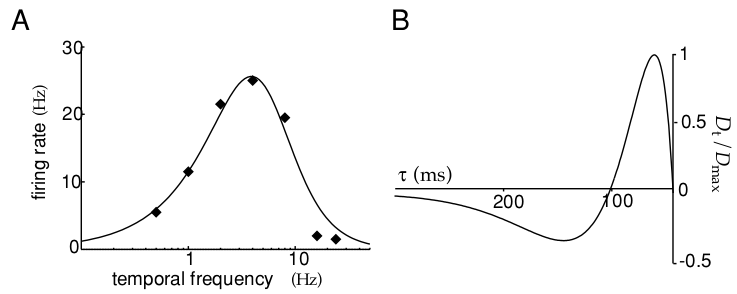
\includegraphics[scale = 0.35]{./png/4-4}
\end{center}
\end{exm}

\begin{exm}
  An interesting test of the notion of optimal coding was carried out by
Dan, Atick, and Reid (1996). They used both natural scene and white-
noise stimuli while recording cat LGN cells. Figure A shows the power spectra of spike trains of cat LGN cells in response to natural scenes (the
movie Casablanca), and figure B shows power spectra in response to
white-noise stimuli. The power spectra of the responses to natural scenes
are quite flat above about $\omega=3$ Hz. In response to white noise, on the
other hand, they rise with $\omega$. This is exactly what we would expect if LGN
cells are acting as temporal whitening filters????????. In the case of natural stimuli,
the whitening filter evenly distributes the output power over a broad fre-
quency range. Responses to white-noise stimuli increase at high frequen-
cies due to the boosting of inputs at these frequencies by the whitening
filter???????.
\begin{center}
  \label{fig:4-5}
  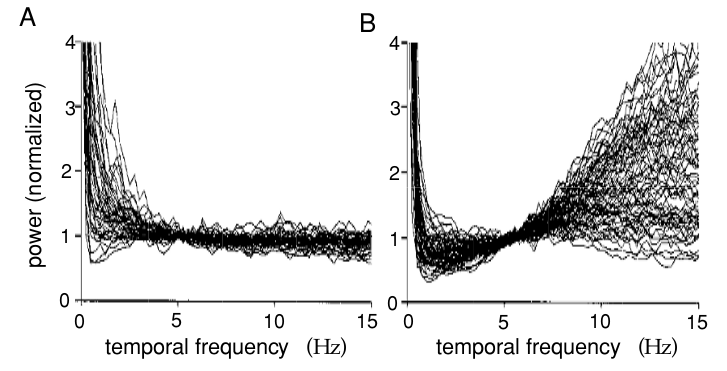
\includegraphics[scale = 0.35]{./png/4-5}
\end{center}
\end{exm}

\subsection{Cortical Coding}
\begin{rem}
  Computational concerns beyond mere linear information transfer are
likely to be relevant at the level of cortical processing of visual
images. For one thing, the primary visual cortex has many more neurons than the
LGN, yet they can collectively convey no more information about the visual world than they receive. As we saw in chapter 2, neurons in primary
visual cortex are selective for quantities, such as spatial frequency and orientation, that are of particular importance in relation to object recognition
but not for information transfer.
\end{rem}
\begin{rem}
  The methods described in
the previous section can be used to understand restricted aspects of recep-
tive fields of neurons in primary visual cortex, namely, the way that their
multiple selectivities are collectively assigned. For example, cells that respond best at high spatial frequencies tend to respond more to low temporal frequency components of images, and vice versa.
\end{rem}
\begin{exm}
 The stimulus power spectrum written as a function of both spatial and
temporal frequency has been estimated as
$\tilde{Q}_{ss}(\vec{\kappa},\omega)\propto 1/(\left| \vec{\kappa} \right|^{2}+\alpha^{2}\omega^{2})$,where $\alpha=0.4$ cycle seconds/degree.This correlation function decreases
both for high spatial and high temporal frequencies. The figure shows how
temporal selectivity for a combined noise and whitening filter, constructed
using this stimulus power spectrum, changes for different preferred spa-
tial frequencies. The basic idea is that components with fairly low stimulus
power are boosted by the whitening filter, while those with very low stim-
ulus power get suppressed by the noise filter. As shown by Li (1996), if a
cell is selective for high spatial frequencies, the input signal rapidly falls
below the noise (treated as white) as the temporal frequency of the input is
increased. As a result, the noise filter of Equation \ref{equ:4.46} causes the temporal
response to be largest at 0 temporal frequency (dashed curve of figure).
If instead the cell is selective for low spatial frequencies, the signal domi-
nates the noise up to higher temporal frequencies, and the whitening filter
causes the response to increase as a function of temporal frequency up to
a maximum value where the noise filter begins to suppress the response
(solid curve in figure)????????.\\

Receptive fields with preference for high spatial
frequency thus act as low-pass temporal filters, and receptive fields with
selectivity for low spatial frequency act as bandpass temporal filters.
\begin{center}
    \label{fig:4-6}
  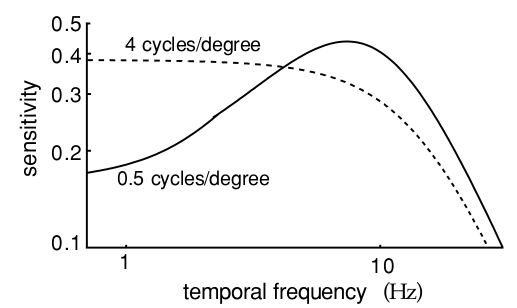
\includegraphics[scale = 0.4]{./png/4-6}
\end{center}
\end{exm}


\begin{exm}
  Similar conclusions can be drawn concerning other joint selectivities. For
example, color-selective (chrominance) cells tend to be selective for low
temporal frequencies, because their input signal-to-noise ratio is lower
than that for broadband (luminance) cells. There is also an interesting
predicted relationship between ocular dominance and spatial frequency
tuning due to the nature of the correlations between the two eyes. Opti-
mal receptive fields with low spatial frequency tuning (for which the in-
put signal-to-noise ratio is high) have enhanced sensitivity to differences
between inputs coming from the two eyes. Receptive fields tuned to inter-
mediate and high spatial frequencies suppress ocular differences?????.
\end{exm}
%%% Local Variables:
%%% mode: latex
%%% TeX-master: "../notesOnFluidMechanics"
%%% End:
